\section{Jump Points}
In the previous section we developed simple rules for pruning neighbours during 
individual node expansions. We now extend this idea in order to define a 
macro-step operator which speeds up optimal search by selectively expanding
only certain nodes on a grid map. We term these nodes \emph{jump points}.

\begin{definition}
\label{def:jump}
A node $x$ is designated a jump point if it satisfies at least one of the following
conditions:
\begin{enumerate}
\item{$x$ is a node which, after pruning, is adjacent to at least one neighbour
whose evaluation is forced according to the rules in Section
\ref{sec:prunestraight} and Section \ref{sec:prunediagonal}.}
\item{$x$ is located on the same row or column of the grid as the goal.}
\item{$x$ has one or more successors which are themselves jump points.}
\end{enumerate}
\end{definition}

Note that we distinguish between a neighbour, which is immediately adjacent to
$x$ on the grid, and a successor which may not be. 
This is a fine but important distinction as in our work a neighbour can be a 
successor but the converse is not necessarily true.
Thus, when expand $x$, we will only consider its successors.

\subsection{Generating Successors}
The process by which we generate the set of successors necessary to expand a
node $x$ is given in Algorithm \ref{alg:successors}.
We start with the pruned set of neighbours immediately adjacent to $x$ (line 2).
Any neighbouring node $n$ whose inclusion into this set is forced, according the 
rules outlined in Section \ref{sec:prunestraight} and Section 
\ref{sec:prunediagonal}, is immediately generated as a successor for $x$ 
(lines 3:4).
We then attempt to defer the generation of each remaining neighbour by seeing if 
we can ``jump'' to another node further away from $x$ but lying in the same 
relative direction to $x$ as $n$ (lines 5:7). For example, if the edge $(x, n)$ constitutes a
straight move travelling \emph{right} from $x$, we look for a jump point among
the nodes immediately to the right of $x$.
If we find such a node, we add it to the set of successors instead of $n$.
In the case where we fail to find a jump point, we add nothing.
The process continues until the set of neighbours for $x$ is exhausted.

\subsection{Finding Jump Nodes}
The general process for searching with jump points can be outlined as 
such: following a pruning operation on some arbitrary node $x$, we defer the immediate 
generation of each remaining neighbour $n$ and, instead, continue travelling in the same direction as from $x$
to $n$.
Thus, we travel past $n$ and instead consider a node $m$ which is two steps
removed from $x$.
At each step, we apply the appropriate pruning rules (straight or
diagonal) and continue this process until we reach an obstacle or identify an 
eventual successor which satisfies certain properties and which we term a 
\emph{jump point}.
If we find such a jump point, we generate it as a successor of $x$; if we do not 
find a jump point, we generate nothing.


\noindent
Figure \ref{fig:pruningrules}(b) shows an example of jump point which satisfies the
first condition of Defintion \ref{def:jump}: here we cannot apply Straight Pruning
Rule 4 as the evaluation of neighbour 3 is forced.
The same is true of the example in Figure \ref{fig:pruningrules}(d): we cannot
apply Diagonal Pruning Rule 3 as the evaluation of neighbour 1 is forced.

\input alg_jumpexpansion

\begin{figure}[tb]
       \begin{center}
		   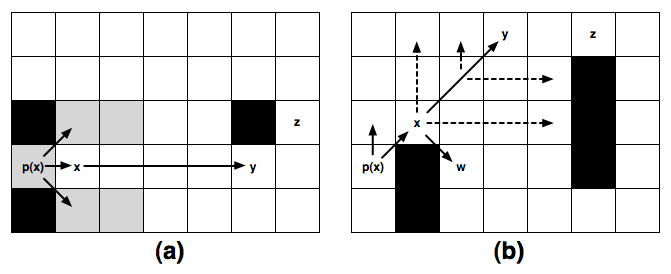
\includegraphics[scale=0.35, trim = 10mm 10mm 10mm 0mm]
			{diagrams/jumppoints.png}
       \end{center}
	\vspace{-3pt}
       \caption{A caption will eventually reside here.}
       \label{fig:jumppoints}
\end{figure}



After pruning, any neighbour which is forced is immediately generated.

\subsection{Optimality}
Sketch: show that each pruning rule discards only neighbours
which cannot belong to the optimal path for the problem at hand.
Then, by induction, demonstrate that jump points have the same 
property. 

Complications:
 - jump points when passing the row or column associated with the goal
 - no jump points at the top of a row/column ending in an obstacle.

